\begin{enumerate}
\item CSV file from a museum, containing 197 artists. %containing 2433 records of artworks by 
\item Linked Data created from the Smithsonian American Art Museum (SAAM) content management system, including over 40,000 artworks and 8,000 artists accessible by a SPARQL endpoint. 
In previous work~\cite{Szekely:2013vq} ~\todo{cite saam-lod github} we mapped the SAAM dataset to the CIDOC CRM ontology~\cite{Doerr:2003:CCR:958671.958678} using \rtworml.
In the demonstration, we are using the SAAM LOD as a proxy for the Linked Data cloud to illustrate the vision of a Linked Data cloud populated with \rtworml models.
\item \rtworml repository containing \rtworml mappings from the Web and made accessible by a \sparql endpoint (separate from the Linked Data endpoint).
\karma provides a component to manage the \rtworml repository (Fig~\ref{fig:model-manager-screenshot}).
\item owl:sameAs links between the datasets' artists generated using LIMES \cite{ngomo2011limes}.
\end{enumerate}
\begin{figure*}[bth]
\begin{center}
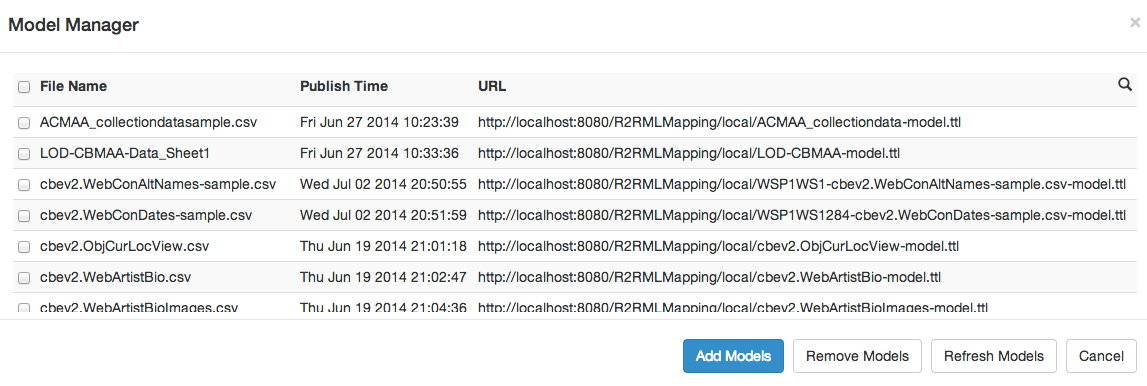
\includegraphics[width=4.8in]{images/3-model-manager.png}
\vspace{-3mm}
\caption{Screenshot of the model manager, showing the \rtworml mappings fetched from the GitHub repository where we shared the mappings for the SAAM dataset}
\vspace{-2mm}
\label{fig:model-manager-screenshot}
\end{center}
\vspace{-1.5em}
\end{figure*}